% Options for packages loaded elsewhere
\PassOptionsToPackage{unicode}{hyperref}
\PassOptionsToPackage{hyphens}{url}
%
\documentclass[
]{article}
\usepackage{amsmath,amssymb}
\usepackage{lmodern}
\usepackage{iftex}
\ifPDFTeX
  \usepackage[T1]{fontenc}
  \usepackage[utf8]{inputenc}
  \usepackage{textcomp} % provide euro and other symbols
\else % if luatex or xetex
  \usepackage{unicode-math}
  \defaultfontfeatures{Scale=MatchLowercase}
  \defaultfontfeatures[\rmfamily]{Ligatures=TeX,Scale=1}
\fi
% Use upquote if available, for straight quotes in verbatim environments
\IfFileExists{upquote.sty}{\usepackage{upquote}}{}
\IfFileExists{microtype.sty}{% use microtype if available
  \usepackage[]{microtype}
  \UseMicrotypeSet[protrusion]{basicmath} % disable protrusion for tt fonts
}{}
\makeatletter
\@ifundefined{KOMAClassName}{% if non-KOMA class
  \IfFileExists{parskip.sty}{%
    \usepackage{parskip}
  }{% else
    \setlength{\parindent}{0pt}
    \setlength{\parskip}{6pt plus 2pt minus 1pt}}
}{% if KOMA class
  \KOMAoptions{parskip=half}}
\makeatother
\usepackage{xcolor}
\usepackage[margin=1in]{geometry}
\usepackage{graphicx}
\makeatletter
\def\maxwidth{\ifdim\Gin@nat@width>\linewidth\linewidth\else\Gin@nat@width\fi}
\def\maxheight{\ifdim\Gin@nat@height>\textheight\textheight\else\Gin@nat@height\fi}
\makeatother
% Scale images if necessary, so that they will not overflow the page
% margins by default, and it is still possible to overwrite the defaults
% using explicit options in \includegraphics[width, height, ...]{}
\setkeys{Gin}{width=\maxwidth,height=\maxheight,keepaspectratio}
% Set default figure placement to htbp
\makeatletter
\def\fps@figure{htbp}
\makeatother
\setlength{\emergencystretch}{3em} % prevent overfull lines
\providecommand{\tightlist}{%
  \setlength{\itemsep}{0pt}\setlength{\parskip}{0pt}}
\setcounter{secnumdepth}{-\maxdimen} % remove section numbering
\ifLuaTeX
  \usepackage{selnolig}  % disable illegal ligatures
\fi
\IfFileExists{bookmark.sty}{\usepackage{bookmark}}{\usepackage{hyperref}}
\IfFileExists{xurl.sty}{\usepackage{xurl}}{} % add URL line breaks if available
\urlstyle{same} % disable monospaced font for URLs
\hypersetup{
  pdftitle={【APLM: homework0929】},
  hidelinks,
  pdfcreator={LaTeX via pandoc}}

\title{\textbf{【APLM: homework0929】}}
\author{}
\date{\vspace{-2.5em}}

\begin{document}
\maketitle

\textbf{\(\mathcal{YiHsin}\;\mathcal{Lu}\)}

\begin{center}\rule{0.5\linewidth}{0.5pt}\end{center}

\hypertarget{exaple-computer-repair-data}{%
\subsection{\texorpdfstring{\textbf{2.3 Exaple: computer repair
data}}{2.3 Exaple: computer repair data}}\label{exaple-computer-repair-data}}

\hypertarget{the-data}{%
\subsubsection{\texorpdfstring{\textbf{1 The
data}}{1 The data}}\label{the-data}}

\begin{itemize}
\tightlist
\item
  x: the length of service calls in minutes
\item
  y: the number of component repaired
\end{itemize}

\begin{verbatim}
##      x  y
## 1   23  1
## 2   29  2
## 3   49  3
## 4   64  4
## 5   74  4
## 6   87  5
## 7   96  6
## 8   97  6
## 9  109  7
## 10 119  8
## 11 149  9
## 12 145  9
## 13 154 10
## 14 166 10
\end{verbatim}

\begin{center}\rule{0.5\linewidth}{0.5pt}\end{center}

\hypertarget{plot}{%
\subsubsection{\texorpdfstring{\textbf{2 Plot}}{2 Plot}}\label{plot}}

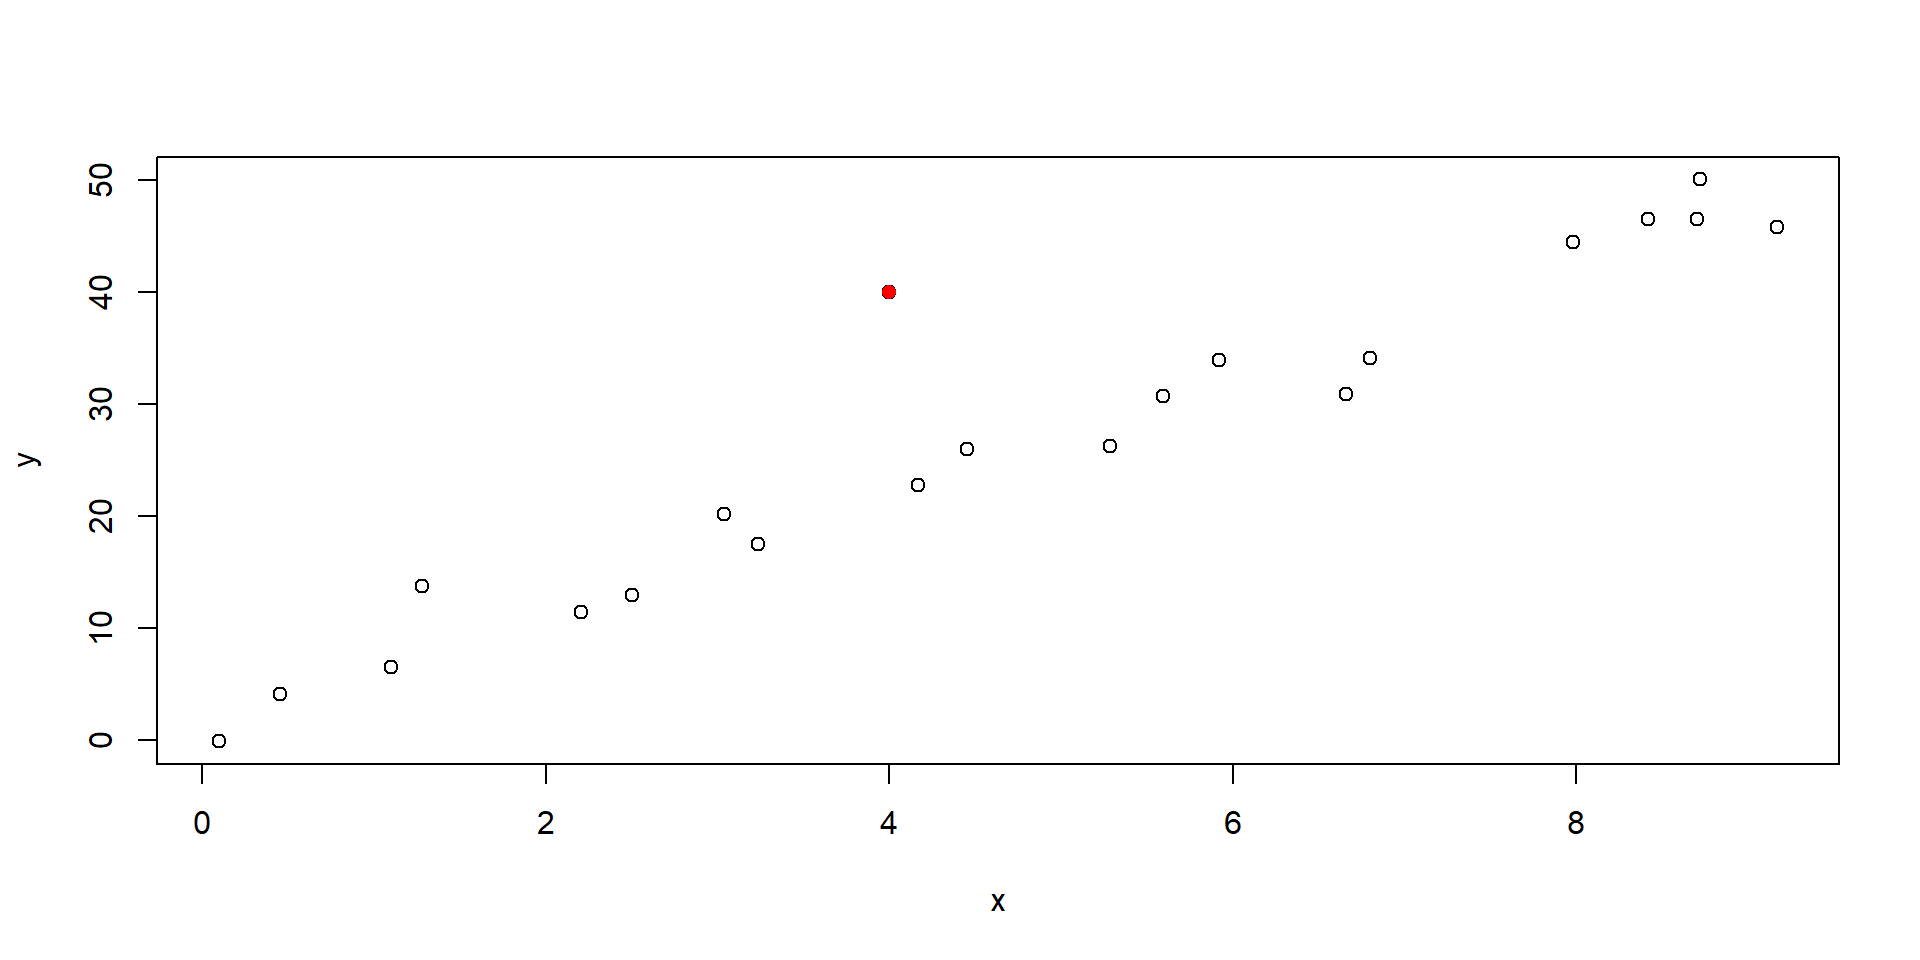
\includegraphics{1013Practice_files/figure-latex/unnamed-chunk-3-1.pdf}

\begin{center}\rule{0.5\linewidth}{0.5pt}\end{center}

\hypertarget{simple-linear-model}{%
\subsubsection{\texorpdfstring{\textbf{3 Simple linear
model}}{3 Simple linear model}}\label{simple-linear-model}}

\begin{verbatim}
## 
## Call:
## lm(formula = y ~ x, data = data1)
## 
## Residuals:
##      Min       1Q   Median       3Q      Max 
## -0.52196 -0.29158  0.04171  0.21589  0.61291 
## 
## Coefficients:
##              Estimate Std. Error t value Pr(>|t|)    
## (Intercept) -0.189594   0.221682  -0.855    0.409    
## x            0.063670   0.002073  30.712 8.92e-13 ***
## ---
## Signif. codes:  0 '***' 0.001 '**' 0.01 '*' 0.05 '.' 0.1 ' ' 1
## 
## Residual standard error: 0.3455 on 12 degrees of freedom
## Multiple R-squared:  0.9874, Adjusted R-squared:  0.9864 
## F-statistic: 943.2 on 1 and 12 DF,  p-value: 8.916e-13
\end{verbatim}

\begin{center}\rule{0.5\linewidth}{0.5pt}\end{center}

\hypertarget{do-t-test}{%
\subsubsection{\texorpdfstring{\textbf{4 Do
t-test}}{4 Do t-test}}\label{do-t-test}}

\begin{itemize}
\item
  \(H_0:\;\beta_0=0\;\) vs \(\;H_1:\;\beta_0\neq 0\)
\item
  p-value = 0.409
\item
  if p-value \textgreater{} \(\alpha\), then we couldn't reject \(H_0\).
  Hence we don't have enough information to say \(\beta_0=0\)
\item
  if p-value \textless{} \(\alpha\), then we reject \(H_0\).Hence
  \(\beta_0\neq0\)
\end{itemize}

\end{document}
